Experiments with cultured neurons on an MEA requires the ability to stimulate and record on all 60 electrodes of the MEA.  The developed Data Acquisition and Stimulation System (DASS) only has the capability of recording data on eight electrodes and outputing four unique stimulation waveforms on those electrodes.  A 60-channel system could be developed by testing and refining, as needed, the hardware and software design principles used by the DASS on a portion of a MEA.  Figure~\ref{fig:System64} shows one possible incarnation of the hardware for a system capable of stimulating and recording with up to 64 electrodes, which is four more channels than necessary for a 60 electrode MEA.

\begin{figure}[htb]
	\begin{singlespace}
	\centering	
		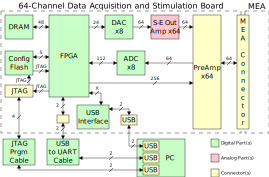
\includegraphics{./figures/System64} 
	\caption{Block diagram of a proposed 64-channel system based on the RTSC board and Electrophysiology Interface board design\label{fig:System64}}
	\end{singlespace}
\end{figure}

The proposed system expands on the circuit designs of the DASS.  A custom PCB connects to the MEA and has a PCI-Express card edge connector socket to interface a PreAmp board to each electrode on the MEA.  The PreAmp voltage output is recorded by eight AD7606 eight-channel ADC components.  Eight AD5678 components contain four 16-bit DACs and four 12-bit DACs each for a total of 64 DAC outputs, and analog amplification circuitry conditions the DAC outputs, providing 64 single-ended stimulation signals to the Preamp boards.  An FPGA on a custom board offers many more IO pins than are available on most development kits; thus, there are likely to be enough IO pins to control the four digital inputs of each PreAmp board without the need for a CPLD for IO expansion.

The FPGA controls the eight AD7606 ADCs and eight AD5678 DACs.  External RAM memory is likely needed to store stimulation waveform data.  A configuration flash memory chip loads the FPGA configuration upon power-up.  A JTAG programming cable eliminates the need for custom microcontroller firmware to load FPGA configurations into the FPGA or configuration flash memory.  A USB to UART cable allows commands to be communicated to the FPGA from the PC with minimal circuitry on the PCB.  And, a microcontroller with a USB PHY allows for fast data transfer of electrode recordings to the PC.

Information that could be acquired by testing this design with the DASS include: confirming whether 12 bits of DAC resolution is sufficient for MEA experiments, determining optimal timing of PreAmp digital control signals, determining which control signals for the ADC and DAC need to be controlled by the FPGA and which can be permanently tied to a logic level, testing data throughput for the USB interface, and, if data transfer speed is found to be insufficient, testing alternative USB2 or USB3 capable microcontrollers.  One area that will need to be tested outside of the current embodiment of the DASS is PCB assembly with ball grid array (BGA) packages: the number of IO pins and logic gates required by a 64-channel system will necessitate the use of a BGA packaged FPGA.
